\chapter{Introduction}
\label{ch:introduction}

% The introduction needs to:
% - Provide a broad background or context to the field or discipline and topic, to orient the reader so that they understand what follows
% - Setup the issue – What’s the problem? What is the scope and limitation existing solutions?
% - State your contributions or argument - What are you bringing that’s new?
% - Signpost and outline the structure of your work

% --- Orienting the reader from the top-down - distributed systems ---
In his book \textit{Distributed Systems: Principles and Paradigms}, Tanenbaum discusses the difficultly in accurately characterising distributed systems and makes allusions to the generally poor definitions often given in the literature, stating that ``none of them [are] satisfactory, and none of them [are] in agreement with any of the others". Distributed systems are so prevalent, it can be difficult to come up with a definition that captures them all. Tanembaum, hence, provides a loose characterisation of a distributed system as a ``collection of independent computers that appears to its users as a single coherent system". This characterisation is sufficient within the context of this work. In this report, we will be focused on exploring decentralised systems, specifically with a peer-to-peer (p2p) architecture and introduce the main output of this project: Butter.\cite{tanenbaum2007distributed}


\section{Background}
\label{sec:background}

In this section we shall be providing some background on distributed systems, distributed architectures and how they can give rise to centralised and decentralised properties, overlay and peer-to-peer networks.

\subsection{Distributed systems \& architectures}
\label{subsec:distributedSystemsArchitectures}

Distributed systems have a few notable characteristics. Firstly, the ``differences between the various computers [constituting the system] and the way in which they communicate are mostly hidden from the user" meaning that the underlying organisation of the system is abstracted away from the user. Secondly, the ``users and applications can interact with a distributed system in a continuous and uniform way, regardless of when and where the interactions take place", which makes them well suited to deliver application services over the internet. Finally, distributed behaviour often lies in-between logical application layers of the system hence it is often referred to as the distributed behaviour middleware.\cite{tanenbaum2007distributed}

\begin{figure}[ht]
    \centering
    \tikzset{edge from parent/.style=
        {draw, edge from parent path={(\tikzparentnode.south)
    -- +(0,-8pt)
    -| (\tikzchildnode)}},
    blank/.style={draw=none}}
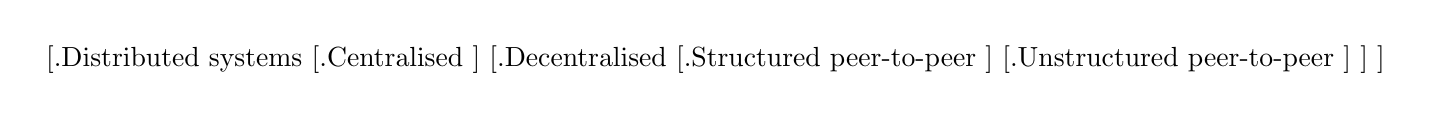
\begin{tikzpicture}
    \matrix
    {
        \node{\Tree
            [.{Distributed systems}
                [.Centralised ]
                [.Decentralised
                    [.{Structured peer-to-peer} ]
                    [.{Unstructured peer-to-peer} ]
                ]
            ]
        };\\
    };
\end{tikzpicture}

    \caption{Distributed systems taxonomy}
    \label{fig:distributed_taxonomy}
\end{figure}

% --- Taxonomy of distributed systems architecture ---
Distributes systems can be organised in several ways depending on how the software components are placed and interact, this leads to an instance of a system architecture\cite{bass2003architecture}. Figure~\ref{fig:distributed_taxonomy} illustrates the taxonomy of distributed systems in terms of the different possible architectures.

% --- Introducing the paradigm of clients and servers ---
In this report, like many other works of distributed systems, we will be thinking in the terms of \textit{clients} initiating connections to fulfil requests from \textit{servers}. A server is a ``process implementing a specific service" such as a database while a ``client is a process that requests a service from a server by sending it a request and subsequently waiting for the server’s reply". Thinking in these terms will help us reason and manage the complexity while discussing the system.\cite{tanenbaum2007distributed}

% --- Introducing centralised vs. decentralised architecture ---
% Vertically distributed architecture
When a system is distributed into logical layers, such as a database, processing components and user-interface, the distribution is vertical as the data flows from one layer to the next\cite{tanenbaum2007distributed}. In this architectural style, the users interface with the service through an endpoint, the top layer of the vertical stack. The user-level clients are distinct, unique and mutually exclusive from the service providing nodes.

% Horizontally distributed architecture
While having a vertical distribution, from a systems' management perspective, can help to logically and physically split system components across machines to provide a service, it is not the only way of organising a distributed system. For instance, distributing clients and servers in such a way that they operate based on their own data set (i.e., their view of the system), thus balancing load, is referred to as horizontal distribution. This distribution style is what gives rise to decentralised systems.\cite{tanenbaum2007distributed}

\subsection{Centralisation \& decentralisation}
\label{subsec:centralisationVsDecentralisation}

% Centralisation
One of the pitfalls of non-distributed systems (i.e. just a single process) or a system with at least one vertical step in its distribution is that they introduce centralisation. Centralisation is when there are unique central processes that others depend on to fulfil a service\cite{raval2016decentralised}. If a serving component of the system fails, clients become unable to access information and interact with the service. This precariousness comes about due to the inherent inter-dependability of the system subcomponents. For example, a typical architecture for a web application includes a vertically distributed database, data processing server and user-interface. The resulting system is distributed yet centralised, as if any one of the subcomponents should fail, e.g. the database, users would be unable to interact with the service. Large, heavily centralised systems consist of few servers relative to the number of clients, hence if a server becomes unavailable, a large number of clients may be unable to function. In some critical systems, where information availability is of paramount importance, a centralised system is at a higher risk of failure making the system less dependable.

\begin{figure}[ht]
    \centering
    \resizebox{\textwidth}{!}{
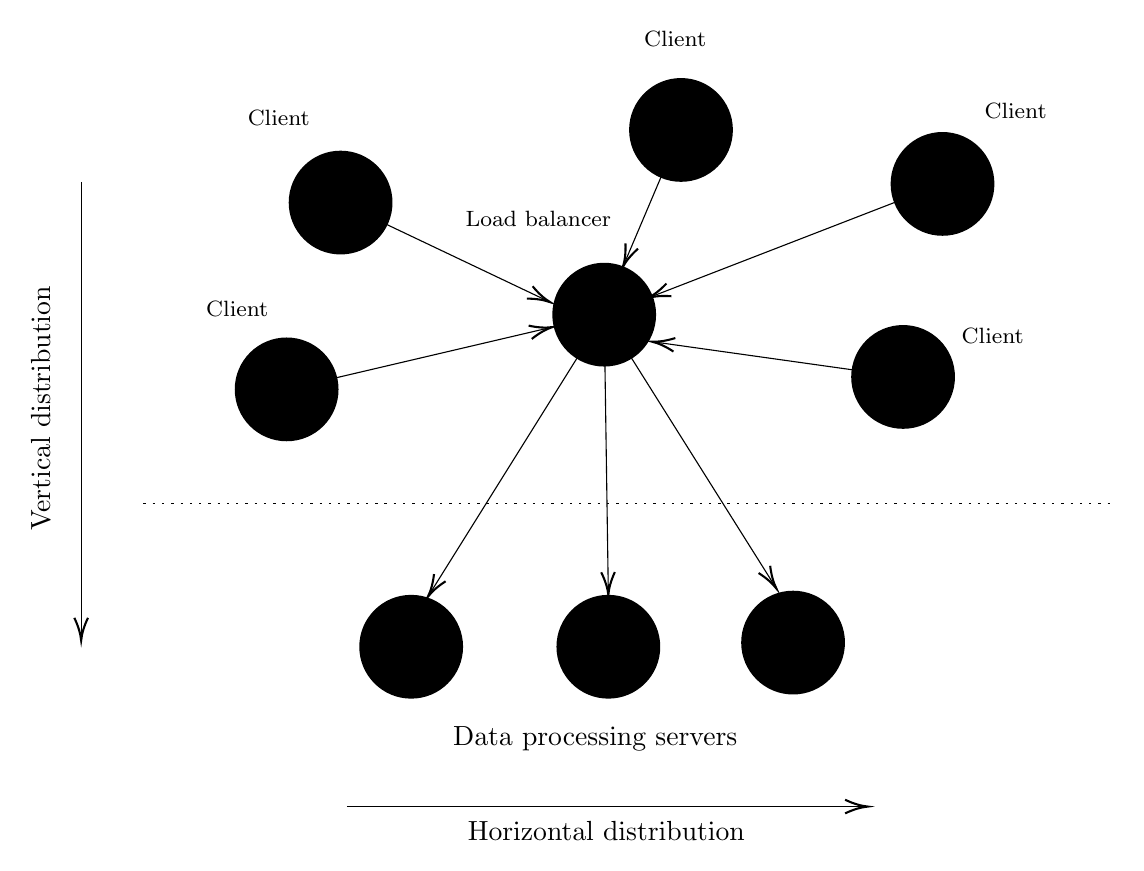
\begin{tikzpicture}[x=0.75pt,y=0.75pt,yscale=-1,xscale=1]
%uncomment if require: \path (0,451); %set diagram left start at 0, and has height of 451

%Shape: Circle [id:dp21625012916250363] 
\draw  [draw opacity=0][fill={rgb, 255:red, 0; green, 0; blue, 0 }  ,fill opacity=1 ] (307,172) .. controls (307,158.19) and (318.19,147) .. (332,147) .. controls (345.81,147) and (357,158.19) .. (357,172) .. controls (357,185.81) and (345.81,197) .. (332,197) .. controls (318.19,197) and (307,185.81) .. (307,172) -- cycle ;
%Shape: Circle [id:dp4205702906990445] 
\draw  [draw opacity=0][fill={rgb, 255:red, 0; green, 0; blue, 0 }  ,fill opacity=1 ] (451,202) .. controls (451,188.19) and (462.19,177) .. (476,177) .. controls (489.81,177) and (501,188.19) .. (501,202) .. controls (501,215.81) and (489.81,227) .. (476,227) .. controls (462.19,227) and (451,215.81) .. (451,202) -- cycle ;
%Shape: Circle [id:dp1834367315754477] 
\draw  [draw opacity=0][fill={rgb, 255:red, 0; green, 0; blue, 0 }  ,fill opacity=1 ] (470,109) .. controls (470,95.19) and (481.19,84) .. (495,84) .. controls (508.81,84) and (520,95.19) .. (520,109) .. controls (520,122.81) and (508.81,134) .. (495,134) .. controls (481.19,134) and (470,122.81) .. (470,109) -- cycle ;
%Shape: Circle [id:dp8062304220658076] 
\draw  [draw opacity=0][fill={rgb, 255:red, 0; green, 0; blue, 0 }  ,fill opacity=1 ] (344,83) .. controls (344,69.19) and (355.19,58) .. (369,58) .. controls (382.81,58) and (394,69.19) .. (394,83) .. controls (394,96.81) and (382.81,108) .. (369,108) .. controls (355.19,108) and (344,96.81) .. (344,83) -- cycle ;
%Shape: Circle [id:dp3524619405588886] 
\draw  [draw opacity=0][fill={rgb, 255:red, 0; green, 0; blue, 0 }  ,fill opacity=1 ] (214,332) .. controls (214,318.19) and (225.19,307) .. (239,307) .. controls (252.81,307) and (264,318.19) .. (264,332) .. controls (264,345.81) and (252.81,357) .. (239,357) .. controls (225.19,357) and (214,345.81) .. (214,332) -- cycle ;
%Shape: Circle [id:dp2671841919001372] 
\draw  [draw opacity=0][fill={rgb, 255:red, 0; green, 0; blue, 0 }  ,fill opacity=1 ] (309,332) .. controls (309,318.19) and (320.19,307) .. (334,307) .. controls (347.81,307) and (359,318.19) .. (359,332) .. controls (359,345.81) and (347.81,357) .. (334,357) .. controls (320.19,357) and (309,345.81) .. (309,332) -- cycle ;
%Shape: Circle [id:dp3753155355544049] 
\draw  [draw opacity=0][fill={rgb, 255:red, 0; green, 0; blue, 0 }  ,fill opacity=1 ] (398,330) .. controls (398,316.19) and (409.19,305) .. (423,305) .. controls (436.81,305) and (448,316.19) .. (448,330) .. controls (448,343.81) and (436.81,355) .. (423,355) .. controls (409.19,355) and (398,343.81) .. (398,330) -- cycle ;
%Shape: Circle [id:dp9331094894799612] 
\draw  [draw opacity=0][fill={rgb, 255:red, 0; green, 0; blue, 0 }  ,fill opacity=1 ] (180,118) .. controls (180,104.19) and (191.19,93) .. (205,93) .. controls (218.81,93) and (230,104.19) .. (230,118) .. controls (230,131.81) and (218.81,143) .. (205,143) .. controls (191.19,143) and (180,131.81) .. (180,118) -- cycle ;
%Shape: Circle [id:dp15130202099269585] 
\draw  [draw opacity=0][fill={rgb, 255:red, 0; green, 0; blue, 0 }  ,fill opacity=1 ] (154,208) .. controls (154,194.19) and (165.19,183) .. (179,183) .. controls (192.81,183) and (204,194.19) .. (204,208) .. controls (204,221.81) and (192.81,233) .. (179,233) .. controls (165.19,233) and (154,221.81) .. (154,208) -- cycle ;
%Straight Lines [id:da6549389594791377] 
\draw    (205,118) -- (304.19,165.14) ;
\draw [shift={(306,166)}, rotate = 205.42] [color={rgb, 255:red, 0; green, 0; blue, 0 }  ][line width=0.75]    (10.93,-3.29) .. controls (6.95,-1.4) and (3.31,-0.3) .. (0,0) .. controls (3.31,0.3) and (6.95,1.4) .. (10.93,3.29)   ;
%Straight Lines [id:da41842174722404835] 
\draw    (179,208) -- (305.05,178.46) ;
\draw [shift={(307,178)}, rotate = 166.81] [color={rgb, 255:red, 0; green, 0; blue, 0 }  ][line width=0.75]    (10.93,-3.29) .. controls (6.95,-1.4) and (3.31,-0.3) .. (0,0) .. controls (3.31,0.3) and (6.95,1.4) .. (10.93,3.29)   ;
%Straight Lines [id:da5248390031839211] 
\draw    (369,83) -- (341.78,147.16) ;
\draw [shift={(341,149)}, rotate = 292.99] [color={rgb, 255:red, 0; green, 0; blue, 0 }  ][line width=0.75]    (10.93,-3.29) .. controls (6.95,-1.4) and (3.31,-0.3) .. (0,0) .. controls (3.31,0.3) and (6.95,1.4) .. (10.93,3.29)   ;
%Straight Lines [id:da3704088342799581] 
\draw    (495,109) -- (354.86,163.28) ;
\draw [shift={(353,164)}, rotate = 338.83] [color={rgb, 255:red, 0; green, 0; blue, 0 }  ][line width=0.75]    (10.93,-3.29) .. controls (6.95,-1.4) and (3.31,-0.3) .. (0,0) .. controls (3.31,0.3) and (6.95,1.4) .. (10.93,3.29)   ;
%Straight Lines [id:da45067791114233546] 
\draw    (476,202) -- (356.98,185.28) ;
\draw [shift={(355,185)}, rotate = 8] [color={rgb, 255:red, 0; green, 0; blue, 0 }  ][line width=0.75]    (10.93,-3.29) .. controls (6.95,-1.4) and (3.31,-0.3) .. (0,0) .. controls (3.31,0.3) and (6.95,1.4) .. (10.93,3.29)   ;
%Straight Lines [id:da675702571699395] 
\draw    (332,172) -- (248.06,306.3) ;
\draw [shift={(247,308)}, rotate = 302.01] [color={rgb, 255:red, 0; green, 0; blue, 0 }  ][line width=0.75]    (10.93,-3.29) .. controls (6.95,-1.4) and (3.31,-0.3) .. (0,0) .. controls (3.31,0.3) and (6.95,1.4) .. (10.93,3.29)   ;
%Straight Lines [id:da19941562676333713] 
\draw    (332,172) -- (333.97,305) ;
\draw [shift={(334,307)}, rotate = 269.15] [color={rgb, 255:red, 0; green, 0; blue, 0 }  ][line width=0.75]    (10.93,-3.29) .. controls (6.95,-1.4) and (3.31,-0.3) .. (0,0) .. controls (3.31,0.3) and (6.95,1.4) .. (10.93,3.29)   ;
%Straight Lines [id:da44186877727070717] 
\draw    (332,172) -- (413.94,302.31) ;
\draw [shift={(415,304)}, rotate = 237.84] [color={rgb, 255:red, 0; green, 0; blue, 0 }  ][line width=0.75]    (10.93,-3.29) .. controls (6.95,-1.4) and (3.31,-0.3) .. (0,0) .. controls (3.31,0.3) and (6.95,1.4) .. (10.93,3.29)   ;
%Straight Lines [id:da00352783652063271] 
\draw  [dash pattern={on 0.84pt off 2.51pt}]  (110,263) -- (578,263) ;
%Straight Lines [id:da8513516782413686] 
\draw    (80,108) -- (80,327) ;
\draw [shift={(80,329)}, rotate = 270] [color={rgb, 255:red, 0; green, 0; blue, 0 }  ][line width=0.75]    (10.93,-3.29) .. controls (6.95,-1.4) and (3.31,-0.3) .. (0,0) .. controls (3.31,0.3) and (6.95,1.4) .. (10.93,3.29)   ;
%Straight Lines [id:da5994970572513846] 
\draw    (208,409) -- (457,409) ;
\draw [shift={(459,409)}, rotate = 180] [color={rgb, 255:red, 0; green, 0; blue, 0 }  ][line width=0.75]    (10.93,-3.29) .. controls (6.95,-1.4) and (3.31,-0.3) .. (0,0) .. controls (3.31,0.3) and (6.95,1.4) .. (10.93,3.29)   ;

% Text Node
\draw (264,121) node [anchor=north west][inner sep=0.75pt]   [align=left] {{\footnotesize Load balancer}};
% Text Node
\draw (159,72) node [anchor=north west][inner sep=0.75pt]   [align=left] {{\footnotesize Client}};
% Text Node
\draw (350,34) node [anchor=north west][inner sep=0.75pt]   [align=left] {{\footnotesize Client}};
% Text Node
\draw (514,69) node [anchor=north west][inner sep=0.75pt]   [align=left] {{\footnotesize Client}};
% Text Node
\draw (503,177) node [anchor=north west][inner sep=0.75pt]   [align=left] {{\footnotesize Client}};
% Text Node
\draw (139,164) node [anchor=north west][inner sep=0.75pt]   [align=left] {{\footnotesize Client}};
% Text Node
\draw (258,369) node [anchor=north west][inner sep=0.75pt]   [align=left] {Data processing servers};
% Text Node
\draw (54.5,277.5) node [anchor=north west][inner sep=0.75pt]  [rotate=-270] [align=left] {Vertical distribution};
% Text Node
\draw (265,415) node [anchor=north west][inner sep=0.75pt]   [align=left] {Horizontal distribution};


\end{tikzpicture}
}

    \caption{Example of a both vertical and horizontally distributed architecture}
    \label{fig:vertHorArch}
\end{figure}

A subtle design to note, is that a system may still be centralised if the underlying server infrastructure is itself horizontally distributed. For example, many cloud services lie behind load balancing servers. The load balancing server does not itself provide the core service but provide a supporting role in balancing server load\cite{rajagopalan2020load}. While the underlying system running the service is horizontally distributed, there is still only a single endpoint with which the client interacts, that of the load balancing server. This is illustrated in Figure~\ref{fig:vertHorArch}, where there is a single publicly available load balancing server which acts an as endpoint for the overall service.

A good example of the risks caused by a centralised service is the `2021 Facebook outage' which made Facebook, WhatsApp and Instagram unavailable for over six hours on October 4th 2021\cite{heath2021facebook}. An engineer made a configuration error while updating a router protocol resulting in the Border Gateway Protocol (BGP)\cite{feamster2005detecting} ``disconnecting Facebook data centres globally"\cite{janardhan2021meta}. This, in turn, prevented Facebook's main DNS server from connecting to other nodes. Facebook has a globally distributed architecture, with backup databases and data processing servers, but users still interact with the services through their domain. If users are unable to resolve the \verb+facebook.com+ domain, they cannot access the underlying service regardless of whether their internal architecture is highly horizontally distributed. This was further worsened by engineers being unable to access the buildings to fix the configuration error as the card authentication system also relied on Facebook's own DNS servers\cite{heath2021facebook}. This case study shows that high levels of centralisation and dependency can be risk-prone and suggests that relying on large centralised cloud services to provide communication services may be unwise.

Decentralisation, which occurs from horizontally distributed architectures, can offer some distinct advantages over a centralised design for delivering certain services. Given that decentralised systems are devoid of hierarchical organisation or centralised control\cite{lua2005survey}, there is no single-point of failure\cite{raval2016decentralised}, however, this comes at a significant cost of performance relative to the centralised equivalent providing the same service. Notably, maintaining information across several nodes comes at the cost of time complexity (as several nodes must process the information), space complexity (as some form of redundancy is often introduced) and most significantly message complexity (as nodes need to communicate with each other to determine their partial views of the system). Designing efficient decentralised protocols is of paramount importance for a decentralised system to effectively deliver its service.

\subsection{Overlay networks}
\label{subsec:overlayNetworks}

\begin{figure}[ht]
    \centering
    % \tikzset{every picture/.style={line width=0.75pt}} %set default line width to 0.75pt        

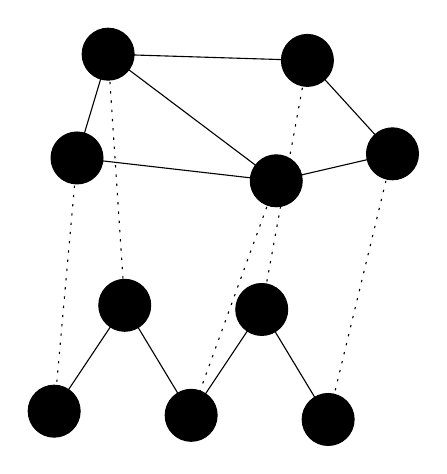
\begin{tikzpicture}[x=0.75pt,y=0.75pt,yscale=-1,xscale=1]
%uncomment if require: \path (0,300); %set diagram left start at 0, and has height of 300

%Shape: Circle [id:dp6061502443078786] 
\draw  [fill={rgb, 255:red, 0; green, 0; blue, 0 }  ,fill opacity=1 ] (125,118.5) .. controls (125,111.6) and (130.6,106) .. (137.5,106) .. controls (144.4,106) and (150,111.6) .. (150,118.5) .. controls (150,125.4) and (144.4,131) .. (137.5,131) .. controls (130.6,131) and (125,125.4) .. (125,118.5) -- cycle ;
%Shape: Circle [id:dp36264343921365794] 
\draw  [fill={rgb, 255:red, 0; green, 0; blue, 0 }  ,fill opacity=1 ] (140,68.5) .. controls (140,61.6) and (145.6,56) .. (152.5,56) .. controls (159.4,56) and (165,61.6) .. (165,68.5) .. controls (165,75.4) and (159.4,81) .. (152.5,81) .. controls (145.6,81) and (140,75.4) .. (140,68.5) -- cycle ;
%Shape: Circle [id:dp9971317502608965] 
\draw  [fill={rgb, 255:red, 0; green, 0; blue, 0 }  ,fill opacity=1 ] (236,71.5) .. controls (236,64.6) and (241.6,59) .. (248.5,59) .. controls (255.4,59) and (261,64.6) .. (261,71.5) .. controls (261,78.4) and (255.4,84) .. (248.5,84) .. controls (241.6,84) and (236,78.4) .. (236,71.5) -- cycle ;
%Shape: Circle [id:dp9106166132377405] 
\draw  [fill={rgb, 255:red, 0; green, 0; blue, 0 }  ,fill opacity=1 ] (277,116.5) .. controls (277,109.6) and (282.6,104) .. (289.5,104) .. controls (296.4,104) and (302,109.6) .. (302,116.5) .. controls (302,123.4) and (296.4,129) .. (289.5,129) .. controls (282.6,129) and (277,123.4) .. (277,116.5) -- cycle ;
%Shape: Circle [id:dp5541002056383258] 
\draw  [fill={rgb, 255:red, 0; green, 0; blue, 0 }  ,fill opacity=1 ] (221,129.5) .. controls (221,122.6) and (226.6,117) .. (233.5,117) .. controls (240.4,117) and (246,122.6) .. (246,129.5) .. controls (246,136.4) and (240.4,142) .. (233.5,142) .. controls (226.6,142) and (221,136.4) .. (221,129.5) -- cycle ;
%Straight Lines [id:da3029168780037723] 
\draw    (152.5,68.5) -- (248.5,71.5) ;
%Straight Lines [id:da46957863774592223] 
\draw    (233.5,129.5) -- (152.5,68.5) ;
%Straight Lines [id:da9097415304582196] 
\draw    (248.5,71.5) -- (289.5,116.5) ;
%Straight Lines [id:da2061802483174313] 
\draw    (137.5,118.5) -- (233.5,129.5) ;
%Straight Lines [id:da9316247214989568] 
\draw    (233.5,129.5) -- (289.5,116.5) ;
%Straight Lines [id:da31757544534246873] 
\draw    (152.5,68.5) -- (137.5,118.5) ;
%Shape: Circle [id:dp39230600009532957] 
\draw  [fill={rgb, 255:red, 0; green, 0; blue, 0 }  ,fill opacity=1 ] (114,240.5) .. controls (114,233.6) and (119.6,228) .. (126.5,228) .. controls (133.4,228) and (139,233.6) .. (139,240.5) .. controls (139,247.4) and (133.4,253) .. (126.5,253) .. controls (119.6,253) and (114,247.4) .. (114,240.5) -- cycle ;
%Shape: Circle [id:dp6725211407093591] 
\draw  [fill={rgb, 255:red, 0; green, 0; blue, 0 }  ,fill opacity=1 ] (148,189.5) .. controls (148,182.6) and (153.6,177) .. (160.5,177) .. controls (167.4,177) and (173,182.6) .. (173,189.5) .. controls (173,196.4) and (167.4,202) .. (160.5,202) .. controls (153.6,202) and (148,196.4) .. (148,189.5) -- cycle ;
%Shape: Circle [id:dp534352110903068] 
\draw  [fill={rgb, 255:red, 0; green, 0; blue, 0 }  ,fill opacity=1 ] (214,191.5) .. controls (214,184.6) and (219.6,179) .. (226.5,179) .. controls (233.4,179) and (239,184.6) .. (239,191.5) .. controls (239,198.4) and (233.4,204) .. (226.5,204) .. controls (219.6,204) and (214,198.4) .. (214,191.5) -- cycle ;
%Shape: Circle [id:dp5705459677432333] 
\draw  [fill={rgb, 255:red, 0; green, 0; blue, 0 }  ,fill opacity=1 ] (246,244.5) .. controls (246,237.6) and (251.6,232) .. (258.5,232) .. controls (265.4,232) and (271,237.6) .. (271,244.5) .. controls (271,251.4) and (265.4,257) .. (258.5,257) .. controls (251.6,257) and (246,251.4) .. (246,244.5) -- cycle ;
%Shape: Circle [id:dp4884732451202879] 
\draw  [fill={rgb, 255:red, 0; green, 0; blue, 0 }  ,fill opacity=1 ] (180,242.5) .. controls (180,235.6) and (185.6,230) .. (192.5,230) .. controls (199.4,230) and (205,235.6) .. (205,242.5) .. controls (205,249.4) and (199.4,255) .. (192.5,255) .. controls (185.6,255) and (180,249.4) .. (180,242.5) -- cycle ;
%Straight Lines [id:da5435068621925384] 
\draw    (160.5,189.5) -- (126.5,240.5) ;
%Straight Lines [id:da40058310101255523] 
\draw    (160.5,189.5) -- (192.5,242.5) ;
%Straight Lines [id:da745960373491508] 
\draw    (226.5,191.5) -- (192.5,242.5) ;
%Straight Lines [id:da9636103089067328] 
\draw    (226.5,191.5) -- (258.5,244.5) ;
%Straight Lines [id:da026025176740933853] 
\draw  [dash pattern={on 0.84pt off 2.51pt}]  (137.5,118.5) -- (126.5,240.5) ;
%Straight Lines [id:da8574677477453254] 
\draw  [dash pattern={on 0.84pt off 2.51pt}]  (152.5,68.5) -- (160.5,189.5) ;
%Straight Lines [id:da45830762125909896] 
\draw  [dash pattern={on 0.84pt off 2.51pt}]  (248.5,71.5) -- (226.5,191.5) ;
%Straight Lines [id:da692101028265002] 
\draw  [dash pattern={on 0.84pt off 2.51pt}]  (233.5,129.5) -- (192.5,242.5) ;
%Straight Lines [id:da20439957038676881] 
\draw  [dash pattern={on 0.84pt off 2.51pt}]  (289.5,116.5) -- (258.5,244.5) ;




\end{tikzpicture}
    \caption{Overlay network of five nodes on top of another network}
    \label{fig:overlay_network}
\end{figure}

% --- What is overlay network ---
An overlay is a logical network that is implemented on top of some underlying network (see Figure~\ref{fig:overlay_network}). There is a one-to-one mapping between the nodes in each layer, i.e., each node in the overlay is associated with a node in the underlying network. The overlay nodes process and forward packets in an application-specific way. There can exist several overlay networks on top of the same underlying network each implementing its own application-specific behaviour and overlays can also be nested, one on top of another.\cite{peterson2012networks}

\subsection{Peer-to-peer systems}
\label{subsec:p2pSystems}

% --- What is peer-to-peer? ---
In this work we will focus on a horizontally distributed system architecture known as peer-to-peer. Peers are ``distributed computational entities each of which are considered equally important in terms of initiating an interaction and each of which provides its own resources"\cite{bass2003architecture}. The peers cooperate and collaborate to provide a service; often to a distributed community of users. In a peer-to-peer system, nodes behaves both as clients and servers. This symmetry supports community resource sharing, however for effective service delivery a fault-tolerant design is required\cite{lua2005survey}.

Peer-to-peer systems are both a ``social and technical phenomenon"\cite{ripeanu2001peer}. They allow for community resource aggregation to share storage space (e.g. Gnutella, Napster, BitTorrent), CPU cycles (e.g. \verb+SETI@Home+), or support collaborative environments (e.g. Groove) hence p2p networks are often used to support community projects that may otherwise be unachievable. There are several factors that have fostered the growth of such systems: first, the low cost and high availability of large numbers of computing and storage resources, second, increased network connectivity\cite{ripeanu2001peer} as well as a desire become less dependent on cloud services\cite{raval2016decentralised}.

Peers form self-organising networks that are `overlayed' on underlying network infrastructure. By their nature, they have the advantage of providing services with ``massive scalability, and fault-tolerance"\cite{lua2005survey}. However, because peer-to-peer systems are decentralised (i.e., fully horizontally distributed) managing data consistency as well as data and service availability is more complex. In many cases it is ``difficult to provide guarantees with peer-to-peer systems because the peers come and go"\cite{bass2003architecture} we refer to this process as `churn'\cite{baldoni2005churn}.

% A peer-to-peer architecture can help address some of the pitfalls of the traditional centralised client-server model such as reducing cost barrier to entry for server infrastructure while being highly scalable, removing single-points of failure and hence targets for malicious attacks and censorship\cite{raval_2016}.

% Include this stuff from the jxta paper as its good!

% There is substance to peer-to-peer technologies as they have the ability to ``greatly increase the utilisation of three valuable and fundamental Internet assets: information, bandwidth, and computing resources All of these are vastly underutilised at this time, partly due to the traditional client-server computing model"\cite{jxta}. 

% They argues it was important to develop p2p systems as ``miles of new fiber have been installed, the new bandwidth gets little use if everyone goes to Yahoo for content and to eBay for auctions. Instead, hot spots just get hotter while cold pipes remain cold"\cite{jxta} and ``new processors and storage devices continue to break records in speed and capacity, supporting more powerful personal devices throughout the network. However, computation continues to accumulate around data centres, which have to increase their workloads at a crippling pace, thus putting immense pressure on space and power consumption"

% ``p2p technologies can adopt a network-based computing style that neither excludes nor inherently depends on centralised control points. This style can enhance the overall reliability and fault tolerance of computing systems"

% Unlike traditional distributed systems, p2p networks aim to aggregate large numbers of computers that join and leave the network frequently and that might not have permanent network (IP) addresses. In pure p2p systems, individual computers communicate directly with each other and share information and resources without using dedicated servers. A common characteristic of this new breed of systems is that they build, at the application level, a virtual network with its own routing mechanisms. The topology of the virtual network and the routing mechanisms used have a significant impact on application properties such as performance, reliability, and, in some cases, anonymity. The virtual topology also determines the communication costs associated with running the p2p application, both at individual hosts and in the aggregate. Note that the decentralised nature of pure p2p systems means that these properties are emergent properties, determined by entirely local decisions made by individual resources, based only on local information: we are dealing with a self-organised network of independent entities.

Note that it is not uncommon to see the terms `node', `peer' and `process' used interchangeably in many works of distributed system and peer-to-peer systems. In this work we will be using the term `node' and `peer' interchangeably.

\subsubsection{Types of peer-to-peer architectures}

As seen in Figure~\ref{fig:distributed_taxonomy}, there exists two types of peer-to-peer architectures; structures and unstructured. In a structured architecture the ``network is constructed using a deterministic procedure"\cite{tanenbaum2007distributed}. Most commonly the network implements a Distributed Hash Table (DHT) where the overlay network ``assigns keys to data items and organises its peers into a graph that maps each data key to a peer"\cite{lua2005survey}. This produces a structured graph which enables efficient information retrieval. Common structured overlay network protocols include Chord\cite{stoica2003chord} and Kadmilia\cite{maymounkov2002kadmilia}.

% Introducing unstructured p2p
In an unstructured overlay network, each node is atomic and indistinguishable from any other node\cite{kalogeraki2003localSearch}. The protocols do not attempt to organise peers, instead constructing a random graph. The resulting network is flat an can also be organised into hierarchical overlays. In this paradigm, randomised algorithms are used for maintaining the network. Each node maintains a list of its neighbours, known hosts, this list is constructed somewhat randomly\cite{tanenbaum2007distributed}. A node makes decision based on its partial view of the network, its immediate known hosts and the information it has collected during its lifetime. The network can at best ``offer probabilities that quality goals will be met, and these probabilities typically increase with the size of the population of peers"\cite{bass2003architecture}.

% Structured vs unstructured
For retrieving information a structured p2p architecture is significantly more efficient than an unstructured architecture\cite{lua2005survey}. In an unstructured overlay, queries for content are spread to a large fraction of peers, and there is no coupling between topology and information location so overlay topology cannot be exploited to improve search efficiency. On the other hand, unstructured networks are better suited to high-churn environments. In so called `churney' environments, nodes frequently join and exit the network ungracefully either because of link or process failure. In a structured network there is an overhead for joining and exiting the network which comes from the `bootstrapping' process where the network re-structures itself to allow the insertion or exit of a node while maintaining a consistent structure. In a community driven service, working over the internet, nodes are often unreliable; frequently joining, leaving, failing, or otherwise ungracefully disconnecting from the network\cite{ripeanu2001peer}. This means that unstructured networks can offer better performance in high churn environments\cite{lua2005survey}.


\section{Motivation \& Goal}
\label{sec:motivationAndgoal}

% --- Introducing motivations ---
% Lack of confidence in cloud services
% Fascinated by the idea of detaching information from infrastructure
% Interested in designing systems that reflect how people deal with information in the real world (i.e. probabilistic vs. deterministic)

This project was mainly motivated by a sense of disillusionment with `cloud' services. Cloud services are ``infrastructure, platforms, or software that are hosted by third-party providers and made available to users through the internet"\cite{redhat2022cloud}. They are often advertised as highly dependable solutions, however, as the Facebook outage example in Section~\ref{subsec:centralisationVsDecentralisation} shows, this is not always the case. The problem of over-reliance on centralised cloud infrastructures is particularly pertinent for community services such as Wikipedia. Wikipedia is a valuable resource of public information hence a decentralised design could be beneficial. It would allow the information to be highly available and devoid of controlling authorities making it much more difficult for malicious users to corrupt or censor information\cite{raval2016decentralised}. Finally, given the information is contributed by the community of users it seems logical to have it hosted by the community as well, giving rise to the notion of community infrastructure.

There is an elegant efficiency to decentralised designs. In heavily centralised, busy network, the servers are expected to handle most of the load, while many clients remain idle. On the other hand, in a peer-to-peer system we can make everyone contribute resources at the benefit of the network. This gives rise to an interesting model of internet consumption where all users are expected to contribute if they want something from a service. Instead of monetizing services through advertising or subscription fees, users collaborate to provide infrastructure. With both open-source software and community hosted infrastructure we have the ability to provide entirely community driven services.

In addition, the design challenge of building a peer-to-peer system provides grounds to explore how information can exist beyond specific infrastructure and to develop probabilistic systems that reflect how people deal with information in the real world. The result is a system that in effect behaves fairly unpredictably hence we need to design algorithms and protocols that maximise the probability of the service being delivered correctly.

Finally instead of simply adopting a pre-existing decentralised network stack such as \verb+libp2p+, we built one because despite the benefits of a decentralised approach, the majority of popular p2p networks include structured elements such as lookup tables, super-peers\cite{garbacki2007optimizing} or Distributed Hash Tables (DHTs). These are introduced primarily to improve network performance by reducing message complexity. However, structured network elements reintroduce some of the pitfalls of the client-server model. This motivated the project's goal of exploring entirely unstructured p2p architectures and their potential for highly-available, fault-tolerant service delivery.


\section{Contribution: Butter}
\label{sec:butterIntroduction}

A node in a peer-to-peer system has to have ``abilities to enable routing, efficient search of data items, selection of nearby peers, redundant storage, permanence, hierarchical naming"\cite{lua2005survey} amongst many other features. In this project, instead of building a specific instance of a decentralised application, where the distributed behaviour is tightly coupled with the application specific logic, we built a framework allowing the isolation of the distributed behaviour middleware. This framework creates a consistent interface for building decentralised applications which is later used for the case studies. In addition, having a highly modular framework allowed for experimenting with different peer-to-peer solutions and protocols. The main output and contribution of this project is the creation of the framework named `Butter', after its approach to managing information availability by `spreading' it across nodes.

\subsection{Problem brief}
\label{subsec:problemBrief}
This section serves as a brief introduction to the main identified problems that a peer-to-peer middleware needs to handle. Greater depth is provided for each problem in Section~\ref{ch:buildingButter}, however, it may be useful to be aware of each of the problems before reading Section~\ref{ch:relatedProjects} and~\ref{ch:projectManagement}.

\begin{itemize}
    \item \textbf{Peer discovery} - How can a node join the network, i.e. form a connection, if it has no pre-existing knowledge of any other nodes?
    \item \textbf{Known host management} - How to manage the existing known host connections in such a way as to improve network performance while dealing with the node's finite resources?
    \item \textbf{NAT Traversal} - How to be visible publicly i.e. have a public facing IP address?
    \item \textbf{Internet discovery} - Same problem as Peer discovery but over the internet
    \item \textbf{Persistent information} - How can information persist beyond the existence of the node hosting it?
    \item \textbf{Information retrieval} - How to quickly and efficiently retrieve a piece of information hosted somewhere on the network?
\end{itemize}


\section{Outline}
\label{sec:outline}
To better understand this report, it is important to note that this project blurs the line between a software engineering project, trying to piece together and implement protocols and technologies to produce a product, and an academic research project, proposing new designs and protocols, experimenting and collecting data. With that said, the report cannot be structured like a pure software engineering report or a research paper. In addition, building and designing a distributed middleware such as Butter requires solving many problems before the system is functional, so, the implementation is broken down into modules for each problem. These modules are introduced in Chapter~\ref{ch:buildingButter} allowing us to present the problem statement, related work, design and implementation as well as testing and evaluation in a self-contained section.

In this report, we will present some similar projects to Butter and discuss how the project was managed. Then we will describe the process of building the Butter framework. Finally, we will discuss some of the case studies, possible future work and conclude. In the conclusion we will summarise the report, discuss the legal, social and ethical considerations for Butter and peer-to-peer systems more broadly and finish with a personal statement on the project from the author.


\begin{table}[h]
    \centering
    \begin{tabular}{|c|c|c|}
        \hline
        \textbf{Problem}                        & \textbf{Butter module} \\
        \hline
        Peer discovery                          & Discovery              \\
        Known host maintenance (edge selection) & Known host management  \\
        NAT traversal and internet discovery    & Wider discovery        \\
        Persistent information                  & Persistent information \\
        Information retrieval                   & Information retrieval  \\
        \hline
    \end{tabular}
    \caption{Core problems and the Butter module that implements the solution}
    \label{tab:prob_module}
\end{table}